\documentclass{article}
\usepackage{graphicx}
\usepackage{cite}
\usepackage{amsmath,amssymb,amsfonts}
\usepackage{algorithmic}
\usepackage{textcomp}
\usepackage{xcolor}
\usepackage{url}
\usepackage{float}
\usepackage{subcaption}

\usepackage{listings}
\usepackage{xcolor}
\usepackage{tabularx}
\usepackage{hyperref}

\usepackage{tikz}
\usetikzlibrary{positioning, shapes.symbols, shapes.geometric, arrows.meta}
\usepackage[
  top=1.3in,
  bottom=1.3in
]{geometry} 




\title{A Dual-Purpose IoT System Using Raspberry Pi Pico W and BMP280: Design and Development of a Weather Station and a Thermal Comfort–Based HVAC Simulation} 
\author{Beatrice Zani, Raffaele Sali, Piero Campos Villagray
\\\footnotesize\href{https://github.com/beazani/Raspberry-Pi-Pico-Indoor-Weather-Station}{github.com/beazani/Raspberry-Pi-Pico-Indoor-Weather-Station}
}
\date{19th December 2025}


\begin{document}

\maketitle

\section{Introduction}
The proliferation of Internet of Things (IoT) technologies has fundamentally transformed environmental monitoring practices, enabling distributed, real-time data collection \cite{atzori2010internet}. Traditional environmental monitoring systems have been characterized by high costs, centralized architectures and limited scalability constraints that modern IoT approaches systematically address through edge computing paradigms and cloud integration.

This project situates itself within the emerging domain of environmental sensing, where computational capabilities are distributed across network nodes rather than centralized on cloud servers. The Raspberry Pi Pico W \cite{vuadan2024advanced} represents a particularly compelling platform for such applications, combining the computational capabilities of the RP2040 microcontroller with integrated Wi-Fi connectivity at a remarkably low cost point \cite{jolles2021broad}.


The choice of temperature and pressure monitoring as the application domain reflects their fundamental importance in multiple contexts. Temperature variations influence everything from building energy efficiency to agricultural productivity, while atmospheric pressure measurements provide insights into weather patterns and altitude-related phenomena.

The system establishes a foundation that can be extended with additional sensors for humidity, air quality, or precipitation monitoring.

\begin{enumerate}
\item \textbf{Sensor Data Collection}

Data was collected using the BMP280 sensor connected to the Pico. The selection of the BMP280 digital sensor represents a deliberate compromise between measurement accuracy, power consumption, cost and interfacing complexity. As a successor to the widely adopted BMP180, the BMP280 offers improved measurement performance with higher resolution for both temperature ($\approx0.01$ °C) and pressure ($\approx0.01$ hPa) compared to its predecessor. It provides typical absolute accuracy of about ±1 °C for temperature and ±1 hPa for pressure, while maintaining low power consumption ($\approx2.7$ µA at 1 Hz) suitable for battery-operated deployments and adds support for both I\textsuperscript{2}C and SPI interfaces \cite{BoschBMP280}.

\item \textbf{Data Processing}

Once acquired, sensor data are processed locally. This processing stage includes numerical rounding, basic sanity checks and temporal labeling using system timestamps. The processed measurements are structured into a standardized data format to ensure consistency across downstream components.
Local data processing serves two key purposes. First, it reduces the amount of raw, unstructured data transmitted over the network, improving communication efficiency. Second, it enables real-time interpretation of sensor readings at the edge, supporting immediate feedback and decision-making without incurring cloud-related latency. This design aligns with edge computing principles, where computation is performed as close as possible to the data source.


\item \textbf{Output Control}

The system provides local feedback through a single onboard LED, which acts as a minimal yet effective output interface for communicating device status. The behaviour of this LED is controlled by a dedicated software module that maps internal system states, such as sensor activity, data transmission events, network connectivity and error conditions, to distinct visual blinking patterns.

In addition to the onboard indicator, two external LEDs (one red and one green) are employed to support the thermal comfort classification task. These LEDs are connected to the microcontroller’s general purpose input/output (GPIO) pins through current-limiting resistors, allowing independent control of each indicator. The external LEDs provide an intuitive representation of the system’s thermal comfort assessment: green for comfort and red for discomfort.
System status information is conveyed through the onboard LED using variations in blinking frequency and duration. A priority based control mechanism ensures that critical conditions, such as alerts and error states, take precedence over routine status indications. This design improves interpretability and reliability of feedback while maintaining a simple and low-cost hardware configuration.
    
\end{enumerate}

\noindent
Within the system, following functionalities were implemented:
\begin{enumerate}
\item \textbf{Wireless Connectivity:}
the Raspberry Pi Pico W is equipped with onboard Wi-Fi, which is leveraged to establish wireless communication with an MQTT broker. In this project, HiveMQ Cloud was employed as the MQTT broker, providing secure, scalable and reliable message delivery. This setup allows real-time transmission of temperature and pressure measurements from the BMP280 sensor, as well as control messages for output devices. 
The MQTT protocol was selected due to its lightweight nature and suitability for constrained IoT devices, ensuring low-latency and efficient communication across the network.

\item \textbf{Cloud Integration:}
collected sensor data and processed metrics are transmitted to a cloud-based data pipeline orchestrated using Node-RED. Node-RED is employed to handle MQTT message ingestion, data parsing and logical routing before storing the processed information in InfluxDB, a time-series database optimized for high-frequency sensor data. This architecture enables persistent storage, efficient querying and structured data management. The stored data is subsequently visualized through Grafana dashboards, providing intuitive insights into environmental conditions and system performance. This integration supports both historical data analysis and near real-time monitoring, while allowing the system to scale seamlessly with additional sensors or nodes.

\item \textbf{Mobile App:} 
the mobile app retrieves data from an API that interfaces with an InFluxDB database. Through predefined API endpoints, the app accesses this information in a structured JSON format. Once received, the app processes the data from each endpoint and presents it as graphs and interactive components, enhancing visualization and making the information more accessible and easier to interpret.

\item \textbf{Edge Machine Learning:}
an embedded trend-based machine learning module is implemented on the Pico W to predict short-term temperature changes and assess thermal comfort. Predictions trigger both the onboard LED patterns enabling autonomous and immediate feedback at the edge without reliance on cloud computation. Trends and predictions are stored and shown in Grafana.

\item \textbf{Thermal Comfort–Based HVAC Simulation:}
a simulated HVAC control mechanism is developed based on a thermal comfort prediction model. The model processes environmental parameters measured by the BMP280 sensor to classify indoor conditions into comfort-related states. Based on the predicted outcome, HVAC adjustments are simulated through visual indicators, where a green LED represents comfort-compliant conditions and a red LED indicates the need for corrective action. This approach enables evaluation of comfort-driven control strategies without the need for physical HVAC hardware, while demonstrating how predictive models can inform adaptive climate control in smart indoor environments.
\end{enumerate}


\section{Architecture} \label{Arch}


%\begin{center}
%\begin{tikzpicture}[every node/.style={draw, rectangle, rounded corners, align=center}]
    % Nodes
%    \node (sensor) at (0,0) {BMP280 Sensor};
%    \node (pico) at (0,-1.5) {Raspberry Pi Pico W};
%    \node (mqtt) at (0,-3) {HiveMQ MQTT Broker};
%    \node (nodered) at (0,-4.5) {Node-RED};
%    \node (influx) at (0,-6) {InfluxDB};
%    \node (grafana) at (-4,-7.5) {Grafana};
%    \node (api) at (4, -7.5) {Flask API};
%    \node (thermal) at (0, -7.5) {Thermal comfort HVAC};
%    \node (app) at (4, -9) {Android Mobile APP};

    % Arrows
%    \draw[->] (sensor) -- (pico);
%    \draw[->] (pico) -- (mqtt);
%    \draw[->] (mqtt) -- (nodered);
%    \draw[->] (nodered) -- (influx);
%    \draw[->] (influx) -- (grafana);
%    \draw[->] (influx) -- (api);
%    \draw[->] (api) -- (app);
%    \draw[->] (influx) -- (thermal);
%\end{tikzpicture}
%\end{center}

\begin{figure}[H]
    \centering
    \includegraphics[width=0.8\textwidth]{img/architecture_pic.png}
    \caption{IoT system architecture}
    \label{fig:architect}
\end{figure}


The architecture in figure \ref{fig:architect} is organized in three primary layers: the \textbf{sensor layer}, the \textbf{networking layer} and the \textbf{data management and visualization layer}. Each layer integrates hardware and software components to enable real time environmental sensing, data processing and feedback.

\subsection{Sensor Layer}

The sensor layer consists of the BMP280 digital sensor connected to the Raspberry Pi Pico W. The sensor provides \textbf{temperature} and \textbf{atmospheric pressure} measurements with high precision, which are essential for environmental monitoring and thermal comfort assessment. The Pico W collects data at regular intervals and performs initial preprocessing, including formatting payloads, adding timestamps and computing latency when necessary. The system also includes output interfaces, consisting of one onboard LED and two external LEDs, to provide immediate visual feedback based on system states and comfort predictions.

\subsection{Networking Layer}

The networking layer is responsible for wireless communication between the Pico W and the cloud infrastructure. The Pico W leverages its onboard Wi-Fi module to connect to the HiveMQ MQTT broker, a cloud-based managed MQTT service designed for scalable and secure message routing in distributed systems \cite{HiveMQ}. MQTT topics are structured to distinguish sensor readings, control signals and predictions of thermal comfort. This protocol ensures lightweight, reliable and low-latency communication suitable for constrained IoT devices. The MQTT protocol will be explained in greater detail in section \ref{methods}.

Node-RED acts as a middleware platform that subscribes to the MQTT topics, orchestrates data processing and manages conditional control logic. Node-RED is a visual, flow-based development tool widely used for integrating IoT data streams and logic without extensive low-level programming \cite{NodeRED}. For example, every 30 seconds Node-RED queries InfluxDB for the latest temperature reading: if the reading exceeds predefined thresholds (too hot or too cold), Node-RED publishes an alert message back to the Pico W via MQTT, enabling real-time feedback on critical conditions.


\subsection{Data Management and Visualization Layer}

The system employs InfluxDB, a time-series database specifically designed for storing and querying high-frequency temporal data. Unlike traditional relational databases, InfluxDB is optimized for metrics, events and sensor readings, providing efficient data compression, retention policies and continuous queries \cite{InfluxDB}. This makes it particularly suitable for IoT applications where large volumes of data are continuously generated. InfluxDB allows fast retrieval of recent measurements, enabling real-time monitoring and analysis of temperature, pressure and thermal comfort prediction data.



For data visualization, the system integrates two solutions:
\begin{itemize}
    \item \textbf{Grafana} \cite{Grafana}, an open-source platform that provides highly configurable dashboards and supports a wide range of data sources, including InfluxDB.
    \item \textbf{Flutter based mobile app}, a personalized mobile application developed by exploiting flask API, which will be explained in section \ref{mob_app}.
\end{itemize} 

Grafana enables the creation of interactive charts, graphs and alerts that help users monitor environmental conditions and assess trends over time. Dashboards can display real-time sensor readings, historical data and thermal comfort status, supporting both immediate feedback and long-term evaluation of system performance. Furthermore, Grafana can be configured to trigger notifications if predefined thresholds are exceeded, complementing the alert logic implemented via Node-RED.

Together, InfluxDB and Grafana provide a robust cloud-based layer for storage, analytics and visualization, ensuring that the system not only processes data locally but also allows remote monitoring and decision-making based on historical and real-time information.

\subsection{Data Flow Summary}

The complete data flow can be summarized as follows:
\begin{enumerate}
    \item The BMP280 sensor measures temperature and pressure.
    \item The Raspberry Pi Pico W collects sensor readings, preprocesses the data and sends it to the HiveMQ MQTT broker.
    \item Node-RED subscribes to the relevant MQTT topics, forwards the readings to InfluxDB for storage and applies logic for alerts.
    \item InfluxDB stores historical and real-time measurements.
    \item Grafana queries InfluxDB to retrieve time-series data and presents it through interactive dashboards for real-time monitoring, trend analysis and alert management. When the monitored temperature exceeds a predefined threshold, Grafana automatically triggers an alert and sends an email notification to inform the user of the anomaly.
    \item If an alert condition is detected (e.g., temperature outside the comfort range), Node-RED publishes a control message via MQTT to the Pico W, which activates the LED indicators.
\end{enumerate}

This architecture enables a seamless integration of edge computing, wireless communication, cloud storage and visualization, supporting both local feedback and long-term analysis.

\section{Methods \& Tools} \label{methods}
This section provides a comprehensive description of the implementation details of the weather monitoring system, outlining the hardware, software, libraries and protocols utilized. This section encompasses sensor data acquisition, local processing on the Raspberry Pi Pico W, wireless transmission via MQTT, middleware orchestration using Node-RED and data storage in InfluxDB for subsequent visualization with Grafana, Android mobile app and thermal comfort prediction.

\subsection{Config file and setup}
The configuration of the entire architecture was developed through the use of a file containing all the relevant parameters required for the connection of the different platforms and protocols. In particular, the file specifies the Wi-Fi network name and password, the MQTT broker details, the topics to be communicated to the broker, the various LED operating configurations for different scenarios, the configuration of the sensors connected to the Raspberry Pi Pico W and the system settings related to timeouts and execution intervals.
Subsequently, the steps for executing the entire pipeline were defined, including connecting the hardware, uploading the project to the hardware, running the main file and activating Node-RED, InfluxDB and Grafana.

\subsection{Sensor readings management}
Environmental data acquisition is performed using a BMP280 sensor, capable of measuring ambient temperature and atmospheric pressure with high accuracy and low power consumption. The sensor is interfaced with the Raspberry Pi Pico W via the I\textsuperscript{2}C communication protocol, which provides a reliable and lightweight bus suitable for embedded and low-power systems.

A dedicated software module, named \texttt{WeatherSensor}, was developed in MicroPython to abstract sensor initialization, data acquisition, error handling and data formatting. During initialization, the module configures the I\textsuperscript{2}C peripheral by specifying the communication channel, Serial Clock Line (SCL) and Serial Data Line (SDA) pins and operating frequency. The SCL line is driven by the master device and provides the clock signal that synchronizes data transfer on the bus, while the SDA line is a bidirectional channel used to transmit and receive data between the master and slave devices. Data on the SDA line is considered valid only when the SCL line is high, ensuring reliable and synchronized communication. This two wire communication scheme reduces pin usage and hardware complexity, making I\textsuperscript{2}C particularly well suited for low-power sensors. The default BMP280 address (0x76) is used, while maintaining compatibility with alternative configurations. 

The sensor driver relies on an open-source MicroPython BMP280 library developed by David Stenwall and distributed through a public GitHub repository \cite{bmp280_library}. This library implements the complete BMP280 datasheet specification, including register-level access, factory calibration data retrieval, oversampling control, power mode selection and digital filtering.

The \texttt{read()} method provides a safe abstraction for retrieving calibrated temperature and pressure values, returning rounded results suitable for transmission and visualization. Error handling mechanisms ensure that invalid reads or disconnected sensors do not propagate corrupted data to higher system layers. Additionally, the \texttt{read\_json()} method encapsulates sensor measurements into a structured dictionary including timestamps and sensor metadata, facilitating seamless integration with the MQTT-based data pipelines and time-series storage systems, which will be described in the following subsections.

To enhance robustness and debugging capabilities, the module includes an I\textsuperscript{2}C bus scanning function that detects connected peripherals and verifies sensor presence. A dedicated test routine performs multiple consecutive readings at fixed intervals to validate sensor stability and correct configuration during deployment.

\subsection{LED management}
The system provides local and immediate feedback through the onboard LED of the Raspberry Pi Pico W, which acts as a minimal yet effective human–machine interface. Given the constrained nature of embedded IoT devices, the LED was chosen as a lightweight output mechanism capable of conveying multiple system states without the need for additional hardware or displays.
LED behavior is encapsulated within a dedicated software component, the \texttt{LEDManager} class. This modular design abstracts low-level GPIO and timing operations, enabling higher-level application logic to trigger visual feedback through system states rather than direct LED control. The manager maps predefined system events, such as Wi-Fi connectivity status, data sending and alert conditions, to distinct blinking patterns characterized by configurable on/off timing parameters. The different blinking patterns and respective states are shown in Table~\ref{tab:led_patterns}.
Blinking behavior is implemented using hardware timers, allowing non-blocking LED control that does not interfere with sensor acquisition, network communication, or data processing tasks.
Priority handling is integrated into the LED management logic to ensure that critical conditions override non-essential indications. In particular, alert-related patterns (e.g., uncomfortable thermal conditions or error states) take precedence over routine operational feedback such as data transmission or connectivity updates. Alert patterns are also automatically extended in duration to increase perceptibility and emphasize abnormal system behavior.
In addition to the onboard LED, the LED management logic supports extensibility toward external indicators. In the implemented system, two external LEDs (red and green) are used to represent the output of the thermal comfort prediction model: the green LED indicates comfortable conditions, while the red LED signals discomfort. These outputs are driven by the same logical framework, ensuring consistency between local feedback and higher-level system decisions.

\begin{table}[H]
\centering
\begin{tabularx}{\textwidth}{l|c|c|X}
\hline
\textbf{State} & \textbf{On} & \textbf{Off} & \textbf{Meaning} \\
\hline
WIFI\_CONNECTING & 0.2 & 0.2 & Device is attempting to connect to Wi-Fi \\
\hline
WIFI\_CONNECTED & 0.05 & 1.0 & Stable Wi-Fi connection (heartbeat pattern) \\
\hline
WIFI\_ERROR & 0.3 & 0.3 & Wi-Fi connection failure \\
\hline
COMFORTABLE & 0.05 & 0.95 & Temperature within comfortable range \\
\hline
UNCOMFORTABLE & 0.15 & 0.15 & Temperature outside comfort range \\
\hline
ALERT & 0.05 & 0.05 & Critical condition requiring attention \\
\hline
\end{tabularx}
\caption{LED blinking patterns and system states}
\label{tab:led_patterns}
\end{table}

\subsection{Wireless connectivity}

Wireless connectivity in the proposed weather monitoring system is achieved through a combination of Wi-Fi networking and the MQTT messaging protocol. This architecture enables reliable, low-latency transmission of sensor data from the Raspberry Pi Pico W to downstream middleware and storage components, while also allowing bidirectional control and feedback.
Network access is handled by a dedicated \texttt{WiFiManager} class, which encapsulates the functionality provided by the MicroPython \texttt{network} module. The Pico W operates in station mode (\texttt{STA\_IF}) and connects to a predefined wireless access point using WPA2 authentication; the password and name of the Wi-Fi to connect to are specified in the \texttt{config.py} file. The connection process includes timeout handling, reconnection attempts and signal strength monitoring based on the received signal strength indicator.
To improve system observability and user feedback, Wi-Fi connection states are visually indicated through the LED management subsystem. During connection attempts, the LED is set to a fast blinking pattern. Once connected, the Wi-Fi manager exposes network configuration parameters such as IP address, gateway, DNS server and signal quality. These parameters can be queried programmatically and included in diagnostic messages or transmitted upstream if required.

\paragraph{MQTT communication model\\}
After establishing network connectivity, sensor data and control messages are exchanged using the Message Queuing Telemetry Transport (MQTT) protocol. MQTT is a lightweight publish–subscribe messaging protocol specifically designed for constrained devices and low-bandwidth, high-latency networks, making it well suited for IoT deployments.
Unlike request–response communication models, MQTT decouples message producers from consumers. Clients publish messages to named topics, while other clients subscribe to topics of interest. Message distribution and coordination are handled by a central broker, which manages client sessions, authentication, message routing and optional message persistence. This architecture allows devices to communicate asynchronously without direct knowledge of one another, improving scalability and fault tolerance.
In the implemented system, the Raspberry Pi Pico W acts as an MQTT client that publishes sensor readings, such as temperature and pressure, to predefined topics (\texttt{weather/temperature, weather/pressure}).
At the same time, it subscribes to control topics that enable remote actuation, including LED state changes and alert triggering. All MQTT communication is performed over TCP to ensure reliable, ordered delivery of messages and Transport Layer Security (TLS) is enabled to provide confidentiality and authentication.

\paragraph{MQTTManager implementation\\}
MQTT functionality is encapsulated within the \texttt{MQTTManager} class, built upon the \texttt{umqtt.robust} library \cite{micropython-umqtt.robust}. This class is responsible for broker connection management, message publishing, subscription handling and callback-based message processing.
Published messages may be transmitted as raw strings or JSON-encoded dictionaries, enabling structured data exchange with middleware components such as Node-RED and InfluxDB. Incoming messages are processed asynchronously through a registered callback function, allowing the device to react to control commands without blocking sensor acquisition or other tasks.
LED-based feedback is tightly integrated with MQTT events: connection attempts, successful connections, data transmission and error states each trigger distinct visual patterns. This coupling between communication state and physical feedback enhances system transparency and simplifies debugging during deployment.

\paragraph{MQTT message structure\\}
MQTT messages, also referred to as control packets, consist of three main components: a fixed header, an optional variable header and a payload. The fixed header is present in all messages and includes the packet type (e.g., CONNECT, PUBLISH, SUBSCRIBE) and the remaining length field. The variable header and payload depend on the specific message type and may include protocol metadata, flags and application data such as sensor readings or control commands. This compact binary format minimizes bandwidth usage and processing overhead, making MQTT suitable for resource-constrained embedded platforms.

\paragraph{HiveMQ broker\\}
In the current implementation, HiveMQ \cite{HiveMQ} was used as the broker. HiveMQ is a cloud-based MQTT broker that manages message routing between publishers and subscribers. Its responsibilities include:
\begin{itemize}
    \item Client connectivity management: ensures devices can connect and maintain sessions.
    \item Message distribution: delivers published messages to all subscribed clients according to topic hierarchy.
    \item Quality of Service (QoS): supports reliable delivery levels.
    \item Optional offline storage: retains messages for clients that are temporarily disconnected.
\end{itemize}

In practice, each sensor reading is published to a structured topic on HiveMQ. Subscribers can then receive these messages in real time. This architecture decouples data producers and consumers, simplifies system scaling and ensures reliable message delivery even in constrained or intermittent networks.


\subsection{Node-RED and InfluxDB}

\subsubsection{Node-RED}

Node-RED \cite{NodeRED} is used to orchestrate the collection, processing and routing of sensor data from MQTT topics. The flow consists of several MQTT input nodes, function nodes for data formatting and outputs for storage and debugging.

\paragraph{Temperature and pressure data flow\\}

MQTT input nodes subscribe to \texttt{weather/temperature} and \texttt{weather/pressure} topics to receive sensor readings from the BMP280. Function nodes parse the payloads, convert them to numeric values or JSON, add metadata (sensor type, location, scenario) and calculate latency if timestamps are available. The processed data is sent to InfluxDB for storage in the created bucket and to debug nodes for monitoring.

\paragraph{Temperature monitoring and alerts\\}

A timer node periodically (every 30 seconds) queries the latest temperature from InfluxDB. A function node checks the value against thresholds (\texttt{TOO\_COLD = 18°C}, \texttt{TOO\_HOT = 25°C}) and generates MQTT messages for LED control as well as InfluxDB entries for alert logging.

\paragraph{Predictions flow}
\begin{itemize}
    \item \textbf{Predictions input:} MQTT input subscribes to \texttt{weather/predictions/\#}.
    \item \textbf{Process prediction:} function node parses prediction payloads, ensures numeric values for all fields, attaches metadata tags and forwards the data to:
    \begin{itemize}
        \item \textbf{InfluxDB node:} stores prediction data in the \texttt{ml\_predictions} measurement.
        \item \textbf{Debug node:} displays prediction payloads for verification.
    \end{itemize}
\end{itemize}

The Node-RED flow integrates MQTT inputs with real-time processing, alert generation and storage in InfluxDB. Debug nodes provide visibility into the data at each stage, enabling monitoring of the IoT system.

\begin{figure}[H]
    \centering \includegraphics[width=0.9\textwidth,height=0.4\textheight]{img/nodered_flow.png}
    \caption{Node-RED flow}
    \label{fig:circle}
\end{figure}

\subsubsection{InfluxDB}
InfluxDB is used as a time-series database to store all sensor measurements. Data from the Node-RED flows is written under the measurement \texttt{weather}. Each entry includes multiple fields, namely \texttt{id}, \texttt{temperature}, \texttt{pressure}, \texttt{latency\_ms}, \texttt{scenario}, \texttt{timestamp} and \texttt{value}. The timestamp represents the time of data insertion, while latency is used to evaluate communication delays. This structure enables efficient querying, filtering and analysis of data over time.
\begin{table}[h]
\centering
\begin{tabular}{ll}
\hline
\textbf{Field} & \textbf{Description} \\
\hline
\texttt{temperature} & Measured temperature value \\
\texttt{pressure} & Measured atmospheric pressure \\
\texttt{latency\_ms} & Message latency \\
\texttt{scenario} & Operating scenario identifier \\
\texttt{timestamp} & Sensor side timestamp \\
\texttt{id} & Message or device identifier \\
\hline
\end{tabular}
\caption{InfluxDB weather measurement fields}
\end{table}

The stored data will later be queried by Grafana for visualization and by a mobile application for real-time monitoring of data and trends.


\subsection{Grafana and mobile app}
\subsubsection{Grafana}

An initial organized view of the information collected in InfluxDB was obtained by creating a dashboard in Grafana. Compared to the mobile app, which is explained in detail in section \ref{mob_app}, this dashboard facilitated real-time monitoring of the entire project during the development and testing phases. Grafana also enabled the development of new metrics, such as air density, calculated using a coefficient of $287.05~\mathrm{J\,kg^{-1}\,K^{-1}}$, based on the temperature and pressure values measured by the sensor \cite{patel2025arduino}.

Figure \ref{fig:grafana} shows part of the dashboard developed, with a comparison between temperature predicted at different times and other metrics. 

\begin{figure}[H]
    \centering
    \includegraphics[width=0.9\textwidth]{img/grafana_dash.png}
    \caption{Dashboard in Grafana to show metrics collected}
    \label{fig:grafana}
\end{figure}


\subsubsection{Mobile app} \label{mob_app}
To retrieve data from InfluxDB and display it in the developed application, a well-defined architecture was followed. The overall architecture, presented earlier in Section~\ref{Arch}, remains the same; however, this section focuses specifically on the data flow from InfluxDB to the API and from the API to the application.

\begin{center}
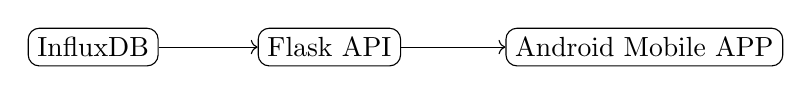
\begin{tikzpicture}[every node/.style={draw, rectangle, rounded corners, align=center}]
    % Nodes
    \node (influx) at (-8,-8) {InfluxDB};
    \node (api) at (-5, -8) {Flask API};
    \node (app) at (-1, -8) {Android Mobile APP};

    % Arrows

    \draw[->] (influx) -- (api);
    \draw[->] (api) -- (app);
\end{tikzpicture}
\end{center}
This subsection of the overall architecture focuses on the data flow dedicated to visualization within the application. It describes how sensor data is collected, processed and ultimately presented to the end user. The following components are involved:
\begin{enumerate}
    \item \textbf{InfluxDB:} serves as the time-series data storage layer, containing all measurements collected from the BMP280 sensor. The sensor transmits data via the Raspberry Pi Pico, which forwards it through a data pipeline involving the HiveMQ MQTT Broker and Node-RED, as described previously. Once ingested into InfluxDB, the data is stored in a structured format and made available for querying by the API.
    \item \textbf{Flask API:} acts as the application layer and middleware interface between the storage and presentation tiers. This RESTful service queries the InfluxDB instance using the Flux query language to retrieve historical and real-time sensor data. The API processes the time-series data and exposes it through standardized JSON endpoints for client consumption. Additionally, it implements token-based authentication mechanisms and supports parameterized queries, allowing flexible retrieval of data over specified time ranges \cite{relan2019building}.

    \item \textbf{Android application:} represents the presentation layer and is developed using the Flutter framework. This cross platform client periodically requests data from the Flask API endpoints, parses the JSON responses and displays the information through a responsive dashboard interface. The interface includes interactive line charts (implemented using the FL Chart library), temperature and environmental data cards and automatic data refresh mechanisms. The application enables users to monitor current sensor readings as well as analyze historical trends through graphical representations of all four measured parameters.

    \begin{figure}[H]
    \centering
    \begin{subfigure}{0.3\textwidth}
        \centering
        \includegraphics[width=\linewidth]{img/SampleImg_App1.jpeg}
        \caption{}
        \label{fig:app_1}
    \end{subfigure}
    %\hfill
    \begin{subfigure}{0.30\textwidth}
        \centering
        \includegraphics[width=\linewidth]{img/SampleImg_App2.jpeg}
        \caption{}
        \label{fig:app_2}
    \end{subfigure}

    \caption{Mobile App visualization}
    \label{fig:App_full}
\end{figure}

\end{enumerate}


\subsection{ML Prediction}

A lightweight trend-based prediction module was implemented to estimate short-term temperature evolution. Instead of relying on computationally expensive machine learning models, the predictor uses a sliding window of recent temperature readings and applies an exponential moving average (EMA) to smooth temperature variations. Based on the smoothed rate of change, the predictor extrapolates future temperature values over configurable time horizons and classifies the thermal trend as \textit{rising}, \textit{falling}, or \textit{stable}. Additional safeguards, such as bounded extrapolation and confidence estimation derived from data availability and signal stability, are included to improve robustness. The resulting predictions are published via MQTT and stored for visualization and analysis.


\subsection{Thermal comfort prediction model in HVAC systems}

To enable real-time thermal comfort assessment using environmental data acquired by the Raspberry Pi Pico and the BMP280 sensor, a machine learning-based thermal comfort prediction model was developed. The model was trained using data from the \textit{ASHRAE Global Thermal Comfort Database II} \cite{ASHRAE_GTC_DBII}, which contains subjective thermal comfort votes together with demographic and environmental information.

\subsubsection{Dataset Preparation}

The original ASHRAE dataset was preprocessed to retain only the variables which were able to collect from the hardware available and some demographic variables that were found relevant. The selected features were:
\begin{itemize}
    \item Age of the occupant.
    \item Sex (encoded as 0 for female and 1 for male).
    \item Air temperature in degrees Celsius.
    \item Thermal comfort score.
\end{itemize}

Age was included as a variable because prior studies have shown that aging affects thermal perception \cite{Farhan2015ThermalComfort}.

The thermal comfort score originally appeared in the dataset in a scale from 1 to 6 and was then converted into a binary target variable in order to formulate a classification problem suitable for real-time control:
\begin{equation}
\text{Comfort} =
\begin{cases}
1, & \text{Comfort score} \geq 5 \\
0, & \text{Comfort score} < 5
\end{cases}
\end{equation}

This binary representation reduces computational complexity while preserving practical usability for HVAC decision-making.

Rows containing missing or non-numeric values in the selected variables were removed. After the preprocessing phase, the dataset contained 13440 observations.  

\subsubsection{Feature Engineering}

To improve model generalization and reduce sensitivity to individual age variations, the continuous age variable was discretized into four age classes:
\begin{table}[H]
\centering
\begin{tabular}{cc}
\hline
\textbf{Age Range (years)} & \textbf{Age Class} \\
\hline
$< 30$ & 0 \\
$30$--$45$ & 1 \\
$45$--$60$ & 2 \\
$\geq 60$ & 3 \\
\hline
\end{tabular}
\caption{Age class definition}
\end{table}

The final input feature vector is defined as:
\begin{equation}
\mathbf{x} = [x_1, x_2, x_3] = [\text{AgeClass}, \text{Sex}, \text{Temperature}]
\end{equation}

\subsubsection{Model Training}

A logistic regression classifier was selected due to its low computational cost, interpretability and suitability for embedded systems \cite{Zheng2024ThermalSensationElderly}. Logistic regression is a statistical and machine-learning method used for binary classification. It models the relationship between input features and the probability of an outcome (such as yes/no or 0/1) by applying a sigmoid (logistic) function to a linear combination of the inputs, producing values between 0 and 1 that can be interpreted as probabilities \cite{lavalley2008logistic}. Prior to training, all input features were normalized using standardization:
\begin{equation}
x_{\text{norm}} = \frac{x - \mu}{\sigma}
\end{equation}
where $\mu$ and $\sigma$ represent the mean and standard deviation computed from the training dataset.

The dataset was divided into training (80\%) and testing (20\%) subsets. Model performance was evaluated using classification accuracy. A custom decision threshold of $0.6$ was selected instead of the default $0.5$ to increase confidence in comfort predictions for HVAC control applications. In fact, $p=0.6$ led to obtaining $accuracy=0.64$ in the test set, higher than the one with $p=0.5$. Choosing a threshold different from $0.5$ is beneficial whenever class imbalance, unequal error costs, or task-specific performance goals make minimizing plain classification error the wrong objective \cite{freeman2008comparison} \cite{hernandez2011threshold}.

\subsubsection{Mathematical Formulation}

The logistic regression model computes a linear combination of the normalized input features:
\begin{equation}
z = \sum_{i=1}^{3} w_i x_i + b
\end{equation}
where $w_i$ are the learned model weights and $b$ is the bias term.

The probability of thermal comfort was obtained using the sigmoid function:
\begin{equation}
P(\text{Comfort}) = \frac{1}{1 + e^{-z}}
\end{equation}

The final classification decision was given by:
\begin{equation}
\text{Comfort} =
\begin{cases}
1, & P(\text{Comfort}) \geq 0.6 \\
0, & P(\text{Comfort}) < 0.6
\end{cases}
\end{equation}

\subsubsection{Model Parameters}

The trained model parameters used for deployment were:
\begin{itemize}
    \item Weights: $w = [0.0605,\ 0.0291,\ -0.2601]$
    \item Bias: $b = 0.5626$
\end{itemize}

The negative weight associated with air temperature indicates that increasing temperature reduces the probability of thermal comfort, which is consistent with established thermal comfort theory.

\subsubsection{Embedded Deployment}

For deployment on the Raspberry Pi Pico, the trained model was reimplemented using basic arithmetic operations and the sigmoid function. Feature normalization was performed using the stored mean and standard deviation values obtained during training. The embedded implementation outputs both the predicted comfort class and the associated probability, enabling real-time thermal comfort estimation and HVAC control. According to the comfort estimation, the LED structure was then built, as explained in section \ref{Arch}.


\section{Evaluation} \label{eval}

The evaluation was focused on analyzing the system performance under different traffic conditions by varying the message payload size and the message transmission rate. The performance was assessed in terms of throughput, latency and reliability.

\subsection{Evaluation Scenarios}

Two evaluation scenarios were defined by focusing on different payload sizes and message transmission rates:

\begin{itemize}
    \item \textbf{Payload Size}
    \begin{itemize}
        \item \textit{Small payload}: publication of a limited set of sensor data fields. Considering the topics, data published were:
        \begin{itemize}
            \item "id": the id of the message
            \item "temperature": the temperature observed
            \item "timestamp": the starting time for latency
            \item "scenario": the label to detect from which scenario the data was obtained, between classic execution, different payload testing and different number of messages testing
            \item "pressure": the pressure observed
        \end{itemize}
        \item \textit{Large payload}: publication of an extended set of sensor data fields. There were included the variables above, with in addition:
        \begin{itemize}
            \item "confidence": the confidence value of the temperature predicted in the following 5 minutes
            \item "change\_per\_sec": the predicted difference per second of the temperature
            \item "change\_per\_min": the predicted difference per minute of the temperature
            \item "change\_per\_hour": the predicted difference per hour of the temperature
            \item "data\_points": the number of observations used to calculate the predictions above
            \item "prediction\_id": the id of the prediction
        \end{itemize}
    \end{itemize}
    \item \textbf{Message Rate}
    \begin{itemize}
        \item \textit{Low number of messages}: sensor data sampled and published every 10 seconds.
        \item \textit{High number of messages}: sensor data sampled and published every 2 seconds.
    \end{itemize}
\end{itemize}

Each of these 4 configurations was executed and tested for a duration of 5 minutes to ensure consistency and comparability of the results.

\subsection{Performance Metrics}

The performance of the system was evaluated using the following metrics:

\subsubsection{Throughput}

Throughput was defined as the number of messages successfully received and processed by Node-RED per minute. It was calculated as follows:

\begin{equation}
    \text{Throughput} = \frac{N_{\text{received}}}{T}
\end{equation}

where $N_{\text{received}}$ represents the total number of messages received during the duration of the test $T$ (in minutes).

\subsubsection{Latency}

Latency measures the end-to-end delay between the moment a sensor observation was generated by the BMP280 and the moment the corresponding data were received by Node-RED and ready for storage in InfluxDB.

It was computed as follows:

\begin{equation}
    \text{Latency} = t_{\text{Node-RED}} - t_{\text{sensor}}
\end{equation}

where $t_{\text{sensor}}$ is the time stamp of observation at the sensor level and $t_{\text{Node-RED}}$ is the time stamp when the data arrive at Node-RED.

\subsubsection{Reliability}

Reliability was evaluated by measuring the number of observations lost during transmission. Each observation was assigned a unique incremental identifier. The number of expected observations was calculated as follows:

\begin{equation}
    N_{\text{expected}} = ID_{\text{last}} - ID_{\text{first}} + 1
\end{equation}

The number of lost observations is then obtained by the following:

\begin{equation}
    N_{\text{lost}} = N_{\text{expected}} - N_{\text{received}}
\end{equation}

A lower number of lost observations indicates greater system reliability.

The results obtained by the evaluation tests are shown in section \ref{results}.

\section{Results} \label{results}

The scenarios explained in section \ref{eval} were tested for 5 minutes. The results obtained are shown by using plots that compare the two configurations within each scenario. 

\subsection{Low/High number of messages scenario} \label{message_rate}

The comparison made in the following figures highlights the impact of different traffic loads on throughput, latency and reliability.

In figure \ref{fig:mess_latency}, the different latency behaviour in the low number of messages and high number of messages configurations can be seen. By looking at the trend of the two lines, no relevant difference can be noticed.

Figure \ref{fig:mess_reliability} highlights the total reliability obtained while running the low number of messages and high number of messages configurations. In the two 5 minutes test no message got lost, leading to have in both configurations the throughput value equals to the ratio between the seconds in a minute and the interval seconds between each observation in each configuration, as shown in figure \ref{fig:mess_throughput}.


\begin{figure}[H]
    \centering
    \includegraphics[width=0.7\textwidth]{img/message_rate_evaluation_latency.png}
    \caption{Latency in the low n° of messages and high n° of messages scenarios}
    \label{fig:mess_latency}
\end{figure}

\begin{figure}[H]
    \centering
    \begin{subfigure}{0.48\textwidth}
        \centering
        \includegraphics[width=\linewidth]{img/message_rate_evaluation_reliability.png}
        \caption{Reliability in the low and high number of messages scenarios}
        \label{fig:mess_reliability}
    \end{subfigure}
    \hfill
    \begin{subfigure}{0.48\textwidth}
        \centering
        \includegraphics[width=\linewidth]{img/message_rate_evaluation_throughput.png}
        \caption{Throughput in the low and high number of messages scenarios}
        \label{fig:mess_throughput}
    \end{subfigure}

    \caption{Message rate evaluation results}
    \label{fig:message_rate_evaluation}
\end{figure}



\subsection{Low/High payload size scenario}

The comparison made in the following figures highlights the impact of payload size on throughput, latency and reliability.

Figure \ref{fig:payload_latency} shows the different latency behaviour while running the small payload size and high payload size configurations. Latency is approximately the same in the two scenarios, with just a single spike in the large payload configuration, reaching more than $5000ms$.

As in the message rate scenario, in section \ref{message_rate}, both configurations received all the messages (figure \ref{fig:payload_reliability}), which can be confirmed by figure \ref{fig:payload_throughput}, where the average throughput obtained while running the small payload size and high payload size configurations is exactly the ratio between the seconds in a minute and the interval seconds between each observation in each configuration.

\begin{figure}[H]
    \centering
    \includegraphics[width=0.7\textwidth]{img/payload_size_evaluation_latency.png}
    \caption{Latency in the small payload and high payload scenarios}
    \label{fig:payload_latency}
\end{figure}

\begin{figure}[H]
    \centering
    \begin{subfigure}{0.48\textwidth}
        \centering
        \includegraphics[width=\linewidth]{img/payload_size_evaluation_reliability.png}
        \caption{Reliability in the small and high payload scenarios}
        \label{fig:payload_reliability}
    \end{subfigure}
    \hfill
    \begin{subfigure}{0.48\textwidth}
        \centering
        \includegraphics[width=\linewidth]{img/payload_size_evaluation_throughput.png}
        \caption{Throughput in the small and high payload scenarios}
        \label{fig:payload_throughput}
    \end{subfigure}

    \caption{Payload size evaluation results}
    \label{fig:payload_evaluation}
\end{figure}




\section{Discussion}
The results obtained from these experiments provide insights into the scalability and robustness of the proposed IoT architecture when subjected to varying data volumes and transmission frequencies.
The evaluation results demonstrate that the proposed IoT system exhibits stable and reliable performance across all tested scenarios, even when subjected to variations in message transmission rate and payload size. The analysis of throughput, latency and reliability provides insight into both the strengths and the limitations of the system under realistic operating conditions.

\subsection{System Strengths}
One of the most significant outcomes of the evaluation is the absence of message loss in all configurations. Both the low and high message rate scenarios, as well as the small and large payload size configurations, achieved perfect reliability during the five minute test intervals. This indicates that the combination of the MQTT protocol, the Raspberry Pi Pico W and the Node-RED–InfluxDB data pipeline is well suited for low to medium intensity IoT workloads. The deterministic throughput observed in all scenarios, which matches the theoretical expected rate based on the sampling interval, further confirms the robustness of the communication and data ingestion architecture.

Latency results also suggest that the system performs consistently under varying traffic conditions. In both the message rate and payload size evaluations, the latency remained largely stable and did not exhibit significant degradation when increasing either the number of messages or the amount of transmitted data. This behavior highlights the effectiveness of MQTT as a lightweight protocol and the ability of Node-RED to efficiently process incoming messages in near real time.

These characteristics make the system particularly suitable for indoor environmental monitoring applications, where sensor data are typically transmitted at moderate rates and timely delivery is more important than ultra-low latency. The observed performance is sufficient to support both real-time visualization through Grafana dashboards and prompt actuation decisions at the edge, such as those required for thermal comfort–based HVAC simulation.

\subsection{Observed Weaknesses and Limitations}

Despite the overall positive performance, some limitations can be identified. In the payload size evaluation, a single latency spike exceeding 5000\,ms was observed in the large payload configuration. While this event did not lead to message loss, it suggests that occasional delays may occur when transmitting more complex payloads that include prediction-related metadata. Such spikes could be attributed to transient network congestion, processing overhead within Node-RED, or buffering effects in the MQTT broker.

Another limitation of the evaluation lies in the controlled nature of the test environment. The experiments were conducted over relatively short durations and under stable network conditions. As a result, the evaluation does not fully capture the behaviour of the system under more demanding scenarios, such as prolonged operation, unstable wireless connectivity, or a significantly higher number of concurrent sensor nodes. Additionally, the current architecture was tested with a single publisher, which limits the assessment of scalability in multi-device deployments.

In addition to the communication and scalability considerations, limitations can be identified in the thermal comfort prediction model itself. The current model is primarily driven by temperature data, combined with static user attributes such as age and sex. While this approach allows for a simplified and computationally lightweight implementation suitable for edge deployment, it inherently restricts the expressiveness and accuracy of the comfort predictions. Thermal comfort is influenced by a broader set of environmental and personal factors, including relative humidity, air velocity, mean radiant temperature and clothing insulation.

The dataset used for training and validation \cite{ASHRAE_GTC_DBII}, includes many of these variables. However, due to hardware constraints, only a subset of the available features could be leveraged in the current implementation. The absence of additional sensors capable of measuring humidity or airflow, for example, limits the ability of the model to fully exploit the richness of the dataset and to generalize across a wider range of indoor conditions. Consequently, the current thermal comfort model accuracy could be significantly improved through the integration of additional sensing modalities and a more feature-complete input representation.

\subsection{Summary}

Overall, the evaluation confirms that the proposed dual-purpose IoT system is robust, reliable and well suited for indoor environmental monitoring and thermal comfort–based HVAC simulation. While minor latency variations were observed under increased payload complexity, the system consistently met its functional requirements, making it an effective platform for both data-driven monitoring and edge-assisted decision-making in smart indoor environments.


\clearpage
\bibliographystyle{unsrt}
\bibliography{references}

\end{document}
